\documentclass{article}

\usepackage[T1]{fontenc}

\usepackage{graphicx}
\graphicspath{ {./obrazki/} }
\usepackage{wrapfig}
\usepackage[export]{adjustbox}
\usepackage{polski}
\usepackage[utf8]{inputenc}
\usepackage[polish]{babel}
\usepackage{gensymb}
\usepackage{xfrac}
\usepackage{anyfontsize}

\title{Pyszności}
\author{Kingi i Mateusza}
\date{2020-03-29}

\begin{document}
    \pagenumbering{gobble}
    \maketitle
    \newpage
    \pagenumbering{arabic}

    % #########################################################################
    % #########################################################################
    % #########################################################################
    \section{Dania obiadowe}
    \medskip
    \subsection{Tortilla}
    \bigskip
    \paragraph{Składniki:}
    \begin{wrapfigure}[1]{r}{0.4\textwidth}
        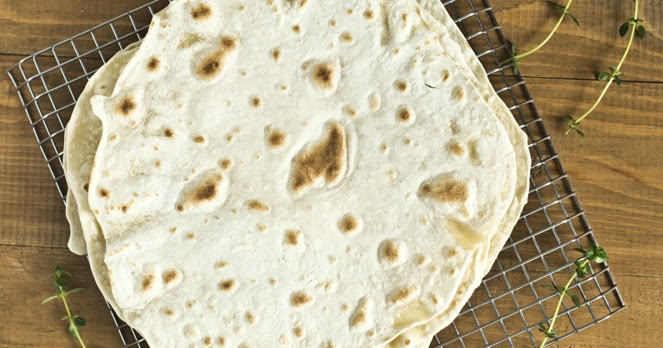
\includegraphics[width=0.4\textwidth]{tortilla.jpg}
    \end{wrapfigure}
    \begin{enumerate}
        \item 250g mąki (tortowa z Łasina)
        \item \sfrac{1}{2} szklanki gorącej wody
        \item \sfrac{1}{2} łyżeczki soli
        \item 2 łyżki smalcu
    \end{enumerate}

    \paragraph{Przygotowanie}
    \begin{enumerate}
        \item Mąkę przesiewamy do miski.
        \item Smalec rozpuszczamy w gorącej wodzie z dodatkiem soli.
        \item Wyrabiamy ciasto przez około 10 minut.
        \item Ciasto dzielimy na około 8-10 części i rozwałkujemy na stolnicy,
            do przezroczystości.
        \item Smażymy placki tortilli na suchej, teflonowej lub ceramicznej
            patelni po ok. 2-4 minuty z każdej storny, aż do uzyskania
            brązowych, rumianych plamek.
        \item Gorące placki nadziewamy farszem i zawijamy.
    \end{enumerate}

    \paragraph{Porada}
    Zimne placki tracą swoją elastyczność, przed zawijaniem należy podgrzać je
    na gorącej, suchej patelni.
    \newpage

    \subsection{Pancakes}
    \bigskip
    \paragraph{Składniki:}
    \begin{wrapfigure}[1]{r}{0.4\textwidth}
        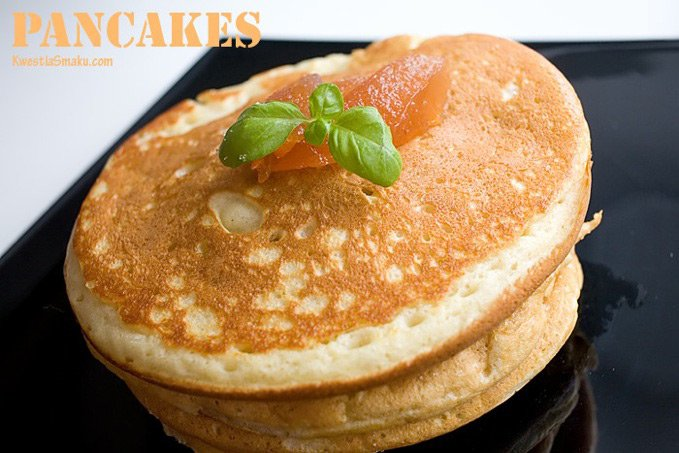
\includegraphics[width=0.4\textwidth]{pancakes.jpg}
    \end{wrapfigure}
    \begin{enumerate}
        \item 2 szklanki mąki
        \item 2 jajka
        \item $1\sfrac{1}{2}$ szklanki mleka
        \item 75 g rozpuszczonego masła
        \item $3\sfrac{1}{2}$ łyżeczki proszku do pieczenia
        \item \sfrac{1}{3} szklanki cukru pudru/cukru brązowego
        \item szczypta soli
    \end{enumerate}

    \paragraph{Przygotowanie}
    \begin{enumerate}
        \item Mąkę przesiać.
        \item Jajka roztrzepać i wymieszać z mlekiem, następnie połączyć z
            pozostałymi składnikami, na końcu dodać masło.
        \item Odstawić na 15 minut.
        \item Smażyć na suchej patelni teflonowej, bez dodatkowego tłuszczu, na
            średnim ogniu, tak aby dać ciastu szansę na wyrośnięcie.
        \item Delikatnie przewrócić na drugą stronę, przy użyciu szerokiej
            łopatki.
    \end{enumerate}
    \newpage

    \subsection{Naleśniki}
    \bigskip
    \paragraph{Składniki:}
    \begin{wrapfigure}[1]{r}{0.4\textwidth}
        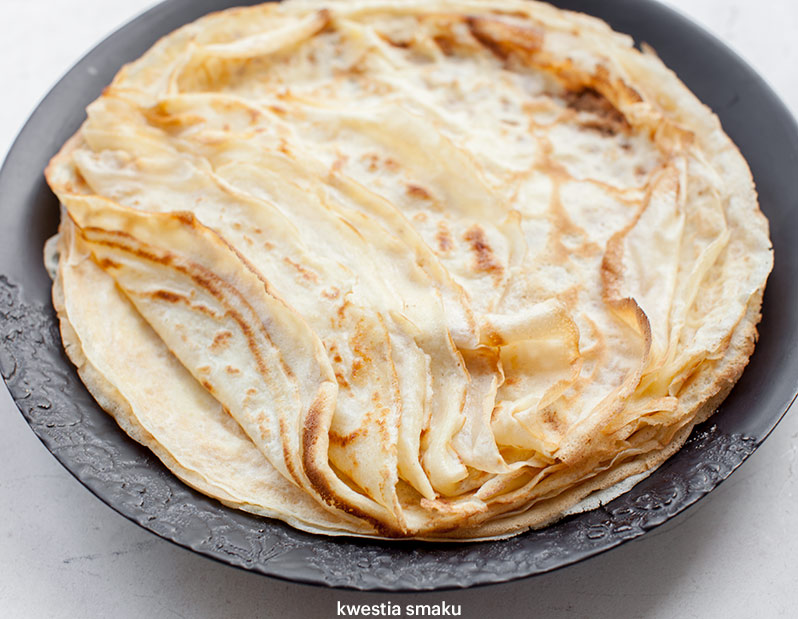
\includegraphics[width=0.4\textwidth]{nalesniki.jpg}
    \end{wrapfigure}
    \begin{enumerate}
        \item 1 szklanka mąki pszennej
        \item 2 jajka
        \item 1 szklanka mleka
        \item \sfrac{3}{4} szklanki wody (najlepiej gazowanej)
        \item szczypta soli
        \item 3 łyżki masła lub oleju roślinnego
    \end{enumerate}

    \paragraph{Przygotowanie}
    \begin{enumerate}
        \item Mąkę wsypać do miski, dodać jajka, mleko, wodę i sól. Zmiksować na
            gładkie ciasto.
        \item Dodać roztopione masło lub olej roślinny i razem zmiksować (lub
            wykorzystać tłuszcz do smarowania patelni przed smażeniem każdego
            naleśnika).
        \item Naleśniki smażyć na dobrze rozgrzanej patelni z cienkim dnem np.
            naleśnikowej. Przewrócić na drugą stronę gdy spód naleśnika będzie
            już ładnie zrumieniony i ścięty.
    \end{enumerate}
    \newpage

    \subsection{Roladki nadziewane pesto z dodatkiem suszonych pomidorów}
    \bigskip
    \paragraph{Składniki:}
    \begin{wrapfigure}[1]{r}{0.4\textwidth}
        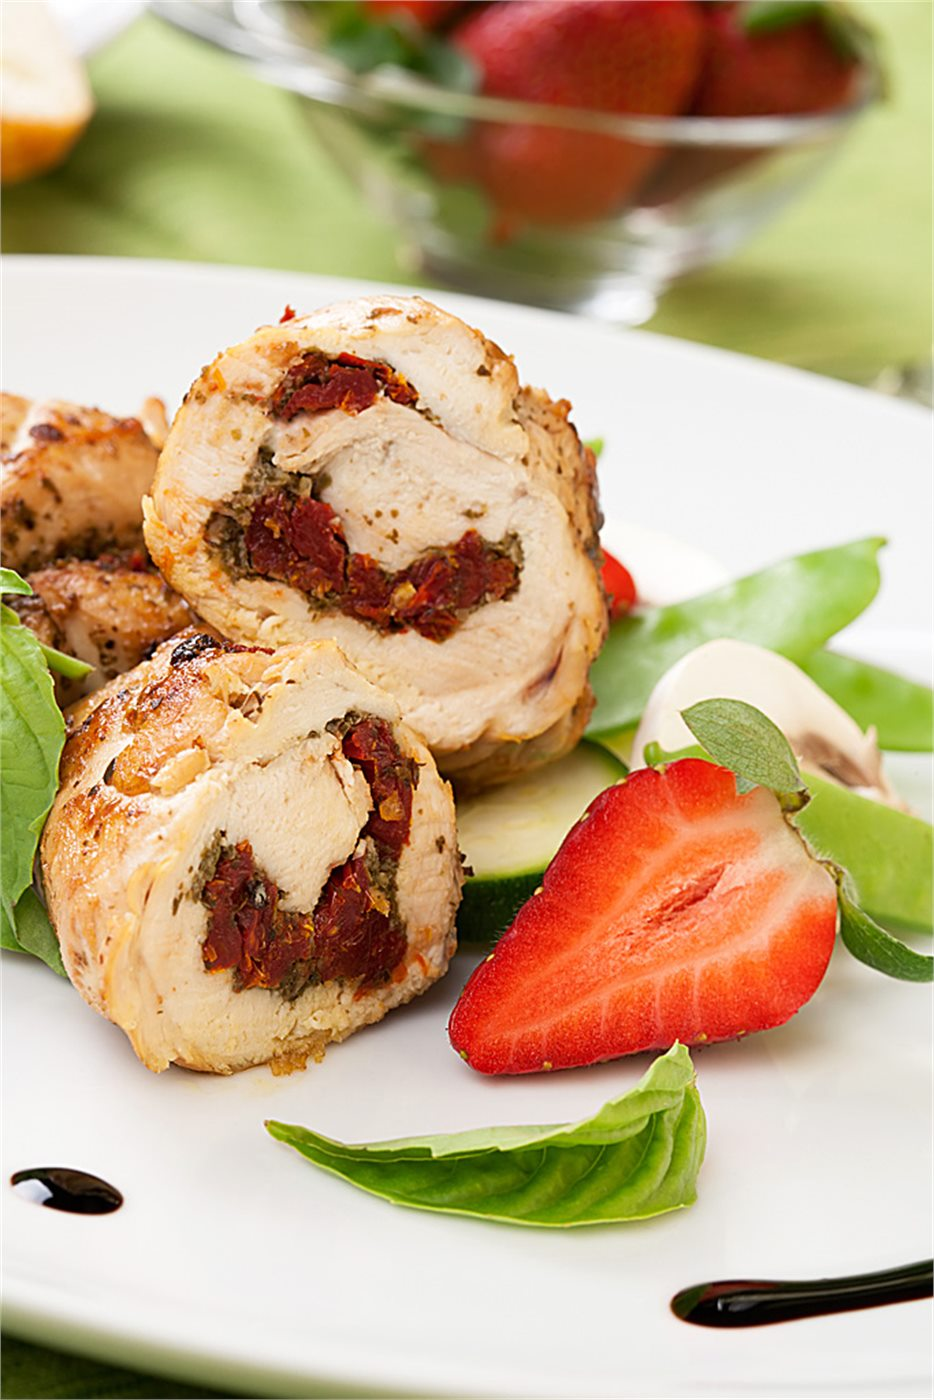
\includegraphics[width=0.4\textwidth]{roladki-z-suszonymi-pomidorami-i-pesto.jpg}
    \end{wrapfigure}
    \begin{enumerate}
        \item Filet z piersi kurczaka - 2,25 porcji (230 g)
        \item Zielone pesto - 2 łyżeczki (35 g)
        \item Pomidory suszone na słońcu - 1,25 garści (35 g)
        \item Ryż brązowy - 0,75 szklanki (120 g)
        \item Pieczarki - 3,25 garści (190 g)
        \item Sól - 2 szczypty (1 g)
        \item Pieprz czarny ziarnisty - 2 szczypty (1 g)
        \item Chilli - 2 szczypty (1 g)
        \item Kurkuma - 2 szczypty (1 g)
    \end{enumerate}

    \paragraph{Przygotowanie}
    \begin{enumerate}
        \item Piersi z kurczaka rozbij tłuczkiem przez folię, tak by nie
            zostawić dziur, posmaruj pesto i dodaj przekrojone na pół plasterki
            suszonych pomidorów. Tak przygotowane mięso zawiń w roladki.
        \item Piekarnik nagrzej do $180\degree$C. W naczyniu żaroodpornym ułóż
            przygotowane roladki. Naczynia nie przykrywaj.
        \item Kiedy mięso delikatnie się zarumieni (po ok. 15–20 minutach)
            podlej je wodą i przykryj naczynie. Piecz mięso jeszcze ok. 10–15
            minut.
        \item W osobnym garnku z grubym dnem podduś na odrobinie wody pieczarki
            razem z przyprawami i dodaj do gotowego mięsa w formie sosu.
        \item Danie podawaj z osobno ugotowanym al dente brązowym ryżem.
    \end{enumerate}
    \newpage

    % #######################################################################
    % #######################################################################
    % #######################################################################
    \section{Desery}
    \medskip
    \subsection{Ciasto czekoladowe}
    \bigskip

    \paragraph{Składniki:}
    \begin{wrapfigure}[3]{r}{0.4\textwidth}
        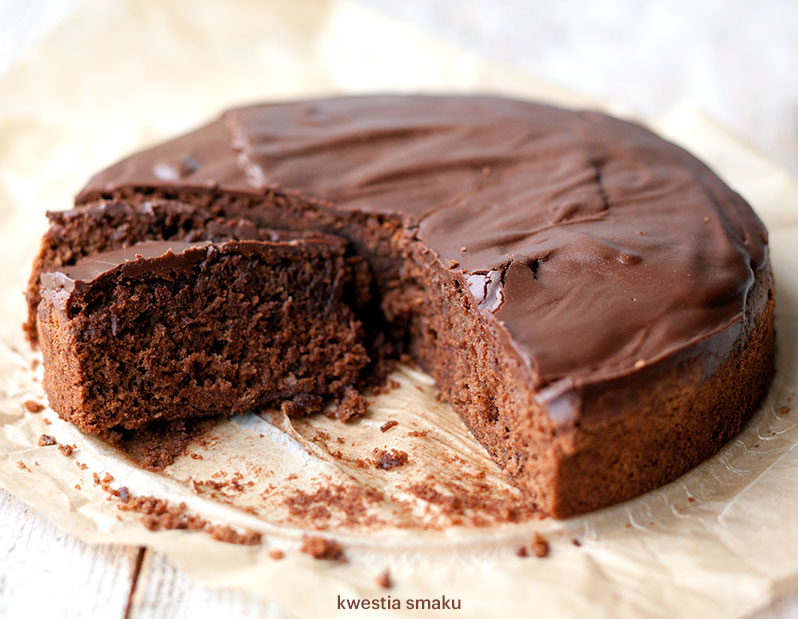
\includegraphics[width=0.4\textwidth]{ciasto_czekoladowe.jpg}
    \end{wrapfigure}
    \begin{enumerate}
        \item 80 g masła
        \item 100 g czekolady deserowej (lekko gorzkiej 50\%) lub po 50 g
            gorzkiej i mlecznej
        \item \sfrac{1}{2} szklanki (125 ml) mleka
        \item 2 jajka
        \item 150 g (\sfrac{3}{4} szklanki) cukru
        \item 150 g (1 szklanka) mąki
        \item 1 łyżeczka proszku do pieczenia
    \end{enumerate}

    \paragraph{Przygotowanie}
    \begin{enumerate}
        \item Jajka ogrzać np. w misce z ciepłą wodą. Dno tortownicy o średnicy
            21 cm wyłożyć papierem do pieczenia, zapiąć obręcz. Piekarnik
            nagrzać do 175 stopni C (góra i dół).
        \item W rondelku umieścić pokrojone masło oraz połamaną na kosteczki
            czekoladę, podgrzewać na minimalnym ogniu ciągle mieszając aż
            składniki się roztopią i otrzymamy gładką masę czekoladową. Odstawić
            z ognia, dodać mleko i wymieszać na gładką masę.
        \item W misce ubić jajka z cukrem (ok. 4 minuty) na puszystą masę. Do
            drugiej miski przesiać mąkę, dodać proszek do pieczenia i dokładnie
            wymieszać. Dodać ubite jajka oraz masę czekoladową, zmiksować na
            minimalnych obrotach miksera lub wymieszać rózgą tylko do połączenia
            się składników w jednolite ciasto.
        \item Wyłożyć je do tortownicy, wstawić do piekarnika i piec przez ok.
            43 minuty do suchego patyczka (w większej niż 21 cm formie, ciasto
            będzie piekło się krócej, ok. 30 - 35 minut, sprawdzamy to
            patyczkiem wetkniętym w środek, czy jest jeszcze obklejony surowym
            ciastem).
    \end{enumerate}
    \newpage


    \subsection{Kruche ciastka z marmoladą}
    \bigskip

    \paragraph{Składniki:}
    \begin{wrapfigure}[3]{r}{0.4\textwidth}
        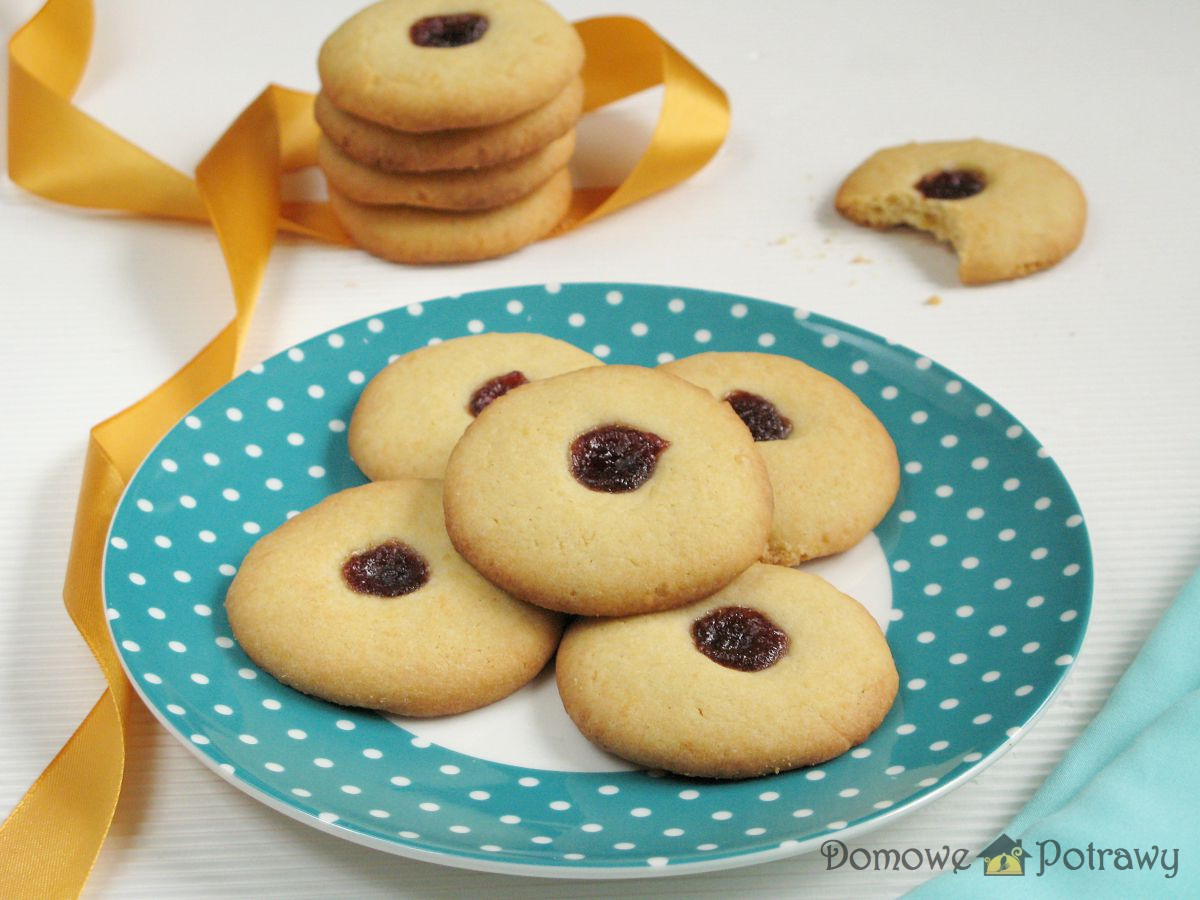
\includegraphics[width=0.4\textwidth]{kruche_ciasteczka_marmolada.jpg}
    \end{wrapfigure}
    \begin{enumerate}
        \item 3 szklanki mąki pszennej
        \item 250 zimnego masła lub margaryny
        \item 2 łyżki smalcu - zamiast smalcu można dać ewentualnie gęstą
            śmietanę 18\%
        \item 3 żółtka
        \item \sfrac{2}{3} szklanki cukru pudru
        \item 1 opakowanie cukru waniliowego (16g)
        \item 2 łyżeczki proszku do pieczenia
        \item szczypta soli
        \item dodatkowo: kilka łyżek marmolady
    \end{enumerate}

    \paragraph{Przygotowanie}
    \begin{enumerate}
        \item Mąkę przesiać przez sito i wsypać do dużej miski. Zimne masło lub
            margarynę pokroić na nieduże kawałki. Wbić żółtka, dodać cukier
            puder, cukier waniliowy, proszek do pieczenia, masło bądź margarynę,
            smalec oraz szczyptę soli. Zagnieść elastyczne ciasto. Podsypać
            mąką, aby się nie kleiło.
        \item Ciasto owinąć w folię spożywczą lub aluminiową i wstawić do
            lodówki na 1 godzinę lub zamrażalnika na 30 minut. Ze schłodzonego
            ciasta odrywać małe kawałeczki wielkości orzecha włoskiego. Formować
            w dłoniach kulki, po czym je spłaszczać. Kłaść na wyłożonej papierem
            do pieczenia blaszce. W każdym ciastku zrobić palcem dziurkę.
        \item Kilka łyżek marmolady przełożyć do woreczka foliowego. Uciąć jeden
            z rogów. Wyciskać odrobinę marmolady do dziurki w ciastkach.
            Ciasteczka piec 15-20 minut w temperaturze $190\degree$C (wcześniej
            nagrzać piekarnik) do lekkiego zarumienia. Studzić na kratce.
            Ciasteczka przechowywać w zamkniętym pojemniku. Zachowują świeżość
            przez
            tydzień.
    \end{enumerate}
    \newpage

    \subsection{Bezy}
    \bigskip
    \paragraph{Składniki:}
    \begin{wrapfigure}[1]{r}{0.4\textwidth}
        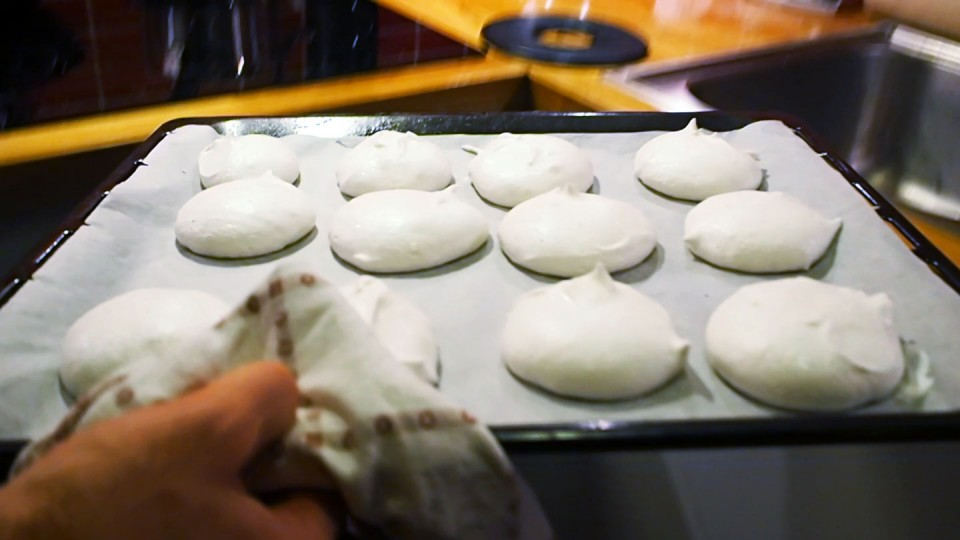
\includegraphics[width=0.4\textwidth]{bezy.jpg}
    \end{wrapfigure}
    \begin{enumerate}
        \item 60g cukru
        \item 60g cukru pudru
        \item białka z 2-3 jajek
        \item szczypta soli
    \end{enumerate}

    \paragraph{Przygotowanie}
    \begin{enumerate}
        \item Wsypać 60g cukru i szczyptę soli do plastikowej miski.
        \item Dodać białka.
        \item Ubić na gęstą, sztywną pianę.
        \item Wmieszać cukier puder do ubitej piany.
        \item Wstawić do piekarnika nagrzanego do $100\degree$C, na
            45min-1h30min w zależności od preferencji i wielkości bez.
    \end{enumerate}
    \newpage

    \subsection{Gofry}
    \bigskip
    \paragraph{Składniki:}
    \begin{wrapfigure}[1]{r}{0.4\textwidth}
        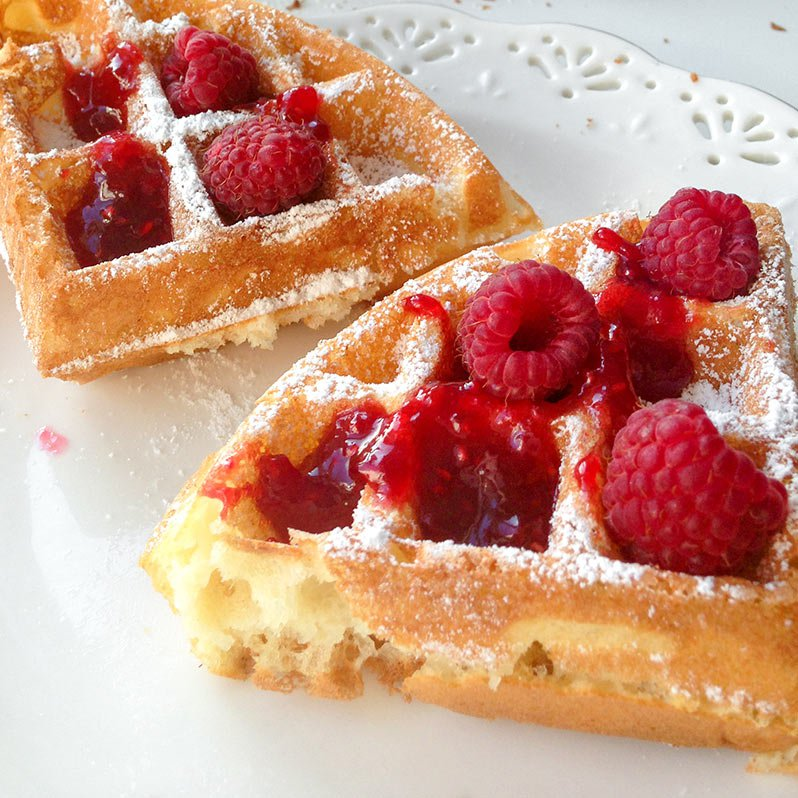
\includegraphics[width=0.4\textwidth]{gofry.jpg}
    \end{wrapfigure}
    \begin{enumerate}
        \item $1\sfrac{1}{2}$ szklanki mąki pszennej
        \item $1\sfrac{1}{2}$ łyżeczki proszku do pieczenia
        \item szczypta soli
        \item 2 łyżeczki cukru pudru lub kryształu
        \item 2 łyżeczki cukru wanilinowego
        \item 2 jaja
        \item \sfrac{1}{2} szklanki oleju roślinnego lub masła
        \item $1\sfrac{1}{3}$ szklanki mleka
    \end{enumerate}

    \paragraph{Przygotowanie}
    \begin{enumerate}
        \item Mąkę wsypać do miski, dodać proszek do pieczenia, sól, cukier,
            cukier wanilinowy. Wszystko wymieszać a następnie dodać jajka, olej
            roślinny oraz mleko. Zmiksować mikserem na gładką masę, tylko do
            połączenia się składników. Ciasto można odstawić aby odpoczęło (na
            około 15 minut), ale nie jest to konieczne.
        \item Rozgrzać gofrownicę. Gofry piec przez około 3 - 3,5 minuty lub
            przez czas podany w instrukcji gofrownicy. Nakładamy ciasto chochlą
            i wypukłą stroną łyżki rozprowadzamy ciasto dokładnie po całej
            powierzchni.
        \item Gofry po upieczeniu odkładać na metalową kratkę. Posypać cukrem
            pudrem i polać syropem klonowym. Lub podawać z ulubionymi dodatkami
            np. marmoladą, dżemem, owocami i bitą śmietaną.
    \end{enumerate}
    \newpage
\end{document}

%    \subsection{Naleśniki}
%    \bigskip
%    \paragraph{Składniki:}
%    \begin{wrapfigure}[1]{r}{0.4\textwidth}
%        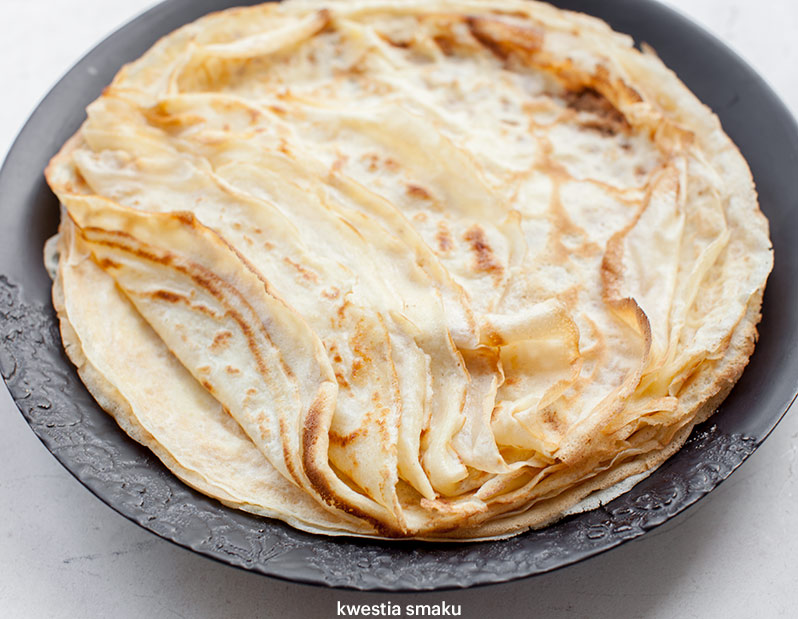
\includegraphics[width=0.4\textwidth]{nalesniki.jpg}
%    \end{wrapfigure}
%    \begin{enumerate}
%    \end{enumerate}
%
%    \paragraph{Przygotowanie}
%    \begin{enumerate}
%    \end{enumerate}
%    \newpage
